\documentclass{../lab}

\labacronym{BRA}
\labtitle{Beta Ray Spectroscopy}

%\newcommand{\NationalBureauofStandards}{http://physics111.lib.berkeley.edu/Physics111/Reprints/BRA/04-Table_for_Analysis_of_Beta_Spectra.pdf}
%\newcommand{\Physics111LibrarySite}{http://physics111.lib.berkeley.edu/Physics111/Reprints/BRA/BRA_index.html}
%\newcommand{\BetaRayApparatus}{http://experimentationlab.berkeley.edu/sites/default/files/images/BRAimage010.gif}
%\newcommand{\Photo-multipliertubeHandbook}{http://physics111.lib.berkeley.edu/Physics111/Equipment_Manuals/RCA_PMT.pdf}
%\newcommand{\BetaandGammaSpectroscopy}{http://physics111.lib.berkeley.edu/Physics111/Reprints/BRA/02-Beta_Ray_Spectrometer.pdf}
%\newcommand{\BetaDecay}{http://physics111.lib.berkeley.edu/Physics111/Reprints/BRA/03-Beta_Decay.pdf}
%\newcommand{\Matalabscripts)}{http://experimentationlab.berkeley.edu/matlabfitting}

\begin{document}

\maketitle

\vspace{3cm}
\centerline{\Huge \bf Experiment is not available at this time.}

\newpage

\tableofcontents

\section{The BETA RAY Experiment (BRA)}

\begin{enumerate}
    \item \textbf{Note that there is NO eating or drinking in the 111-Lab anywhere, except in rooms 282 \& 286 LeConte on the bench with the BLUE stripe around it.} Thank you -- the Staff.
\end{enumerate}

Radioactive decay of nuclei by emitting beta rays (electrons) is a fundamental phenomenon of nuclear physics. In this experiment you will measure the momenta of beta rays emitted by radioactive cesium. By studying the number of electrons emitted as a function of momentum you will obtain information about the nuclear decay processes.

You will setup the experiment using a LabView Program and view the data with histograms. If you know what you are doing and make no mistake, you can complete the data-taking within a week. Data analysis is not trivial; you will need to plot a number of graphs, and analyze them. You will need to learn nuclear physics of beta decay and internal conversion by reading some of the reference materials listed in this write-up. You will also learn about particle motion in a magnetic field, mass spectrometer, amplifiers, single-channel analyzer, counting statistics, computer control of data-taking, and how to handle radioactive materials safely. Once you set up the electronics, data -taking is computer controlled. You use Matlab to analyze the data. There are Matlab scripts already written to help in the analysis (see Matlab fitting).

\begin{enumerate}
    \item Pre-requisites: None

    \item Days Allotted for the Experiment: 6
\end{enumerate}

This lab will be graded 30\% on theory, 30\% on technique, and 40\% on analysis. For more information, see the \href{\AdvancedLabSyllabus}{\textbf{Advanced Lab Syllabus}}.

Comments: E-mail \href{\MailDonOrlando}{\textbf{Don Orlando}}

\section{The Beta Ray Spectroscopy Experiment Photos}

\begin{figure}[H]
\captionsetup{justification=centering}
\minipage{0.32\textwidth}
  \href{http://experimentationlab.berkeley.edu/sites/default/files/images/Bra_1.jpg}{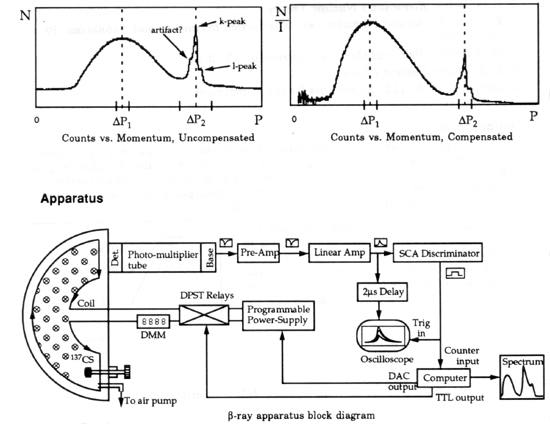
\includegraphics[height=100pt,keepaspectratio]{images/Bra_1.jpg}}
  \caption{Beta Ray \\ Apparatus Block Diagram \\ \href{http://experimentationlab.berkeley.edu/sites/default/files/images/Bra_1.jpg}{Click here to see larger picture}}
  \label{fig:BRayBlock}
\endminipage\hfill
\minipage{0.32\textwidth}
 \href{http://experimentationlab.berkeley.edu/sites/default/files/images/BRA_Rack_1.jpg}{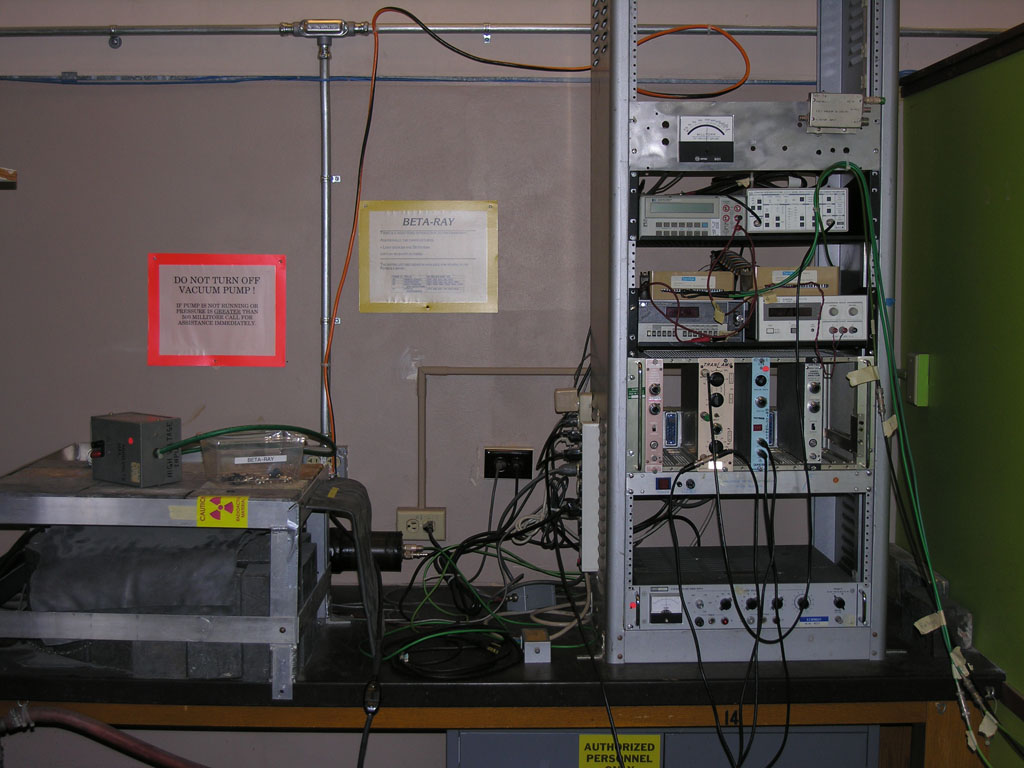
\includegraphics[height=100pt,keepaspectratio]{images/BRA_Rack_1.jpg}}
  \caption{Beta \\ Ray Apparatus\\ \href{http://experimentationlab.berkeley.edu/sites/default/files/images/BRA_Rack_1.jpg}{Click here to see larger picture}}\label{fig:BRayApparatus}
\endminipage\hfill
\minipage{0.32\textwidth}
\centering
  \href{http://experimentationlab.berkeley.edu/sites/default/files/images/RCA6655A_PMT_3.jpg}{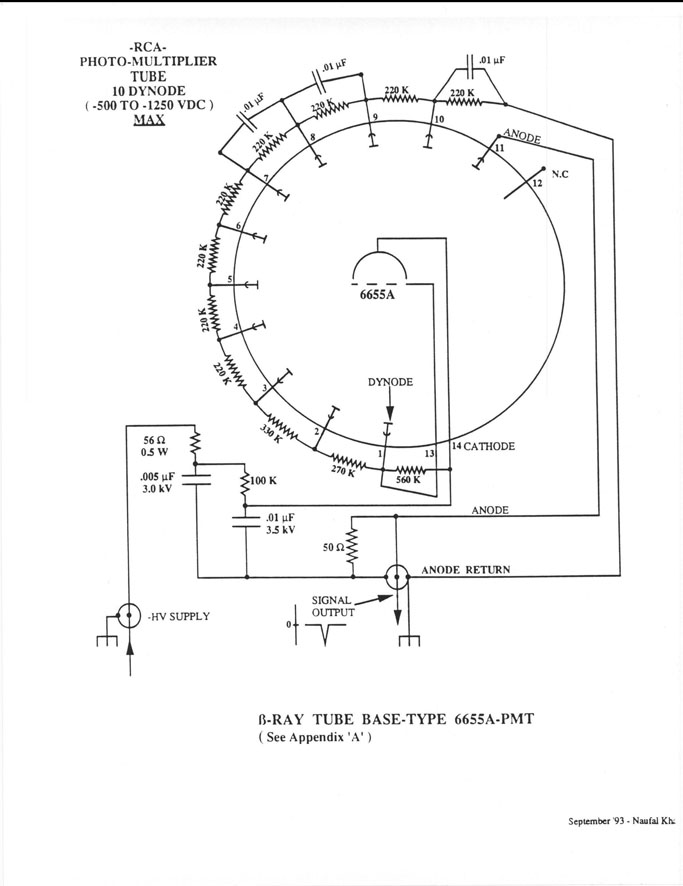
\includegraphics[height=100pt,keepaspectratio]{images/RCA6655A_PMT_3.jpg}}
  \caption{Circuit Diagram \\ of the PMT Base \\
  \href{http://experimentationlab.berkeley.edu/sites/default/files/images/RCA6655A_PMT_3.jpg}{Click here to see larger picture}}
  \label{fig:BRayTube}
\endminipage
\end{figure}

\begin{figure}[H]
\captionsetup{justification=centering}
\minipage{0.49\textwidth}
\centering
  \href{http://experimentationlab.berkeley.edu/sites/default/files/images/Lead_Brick_Shield.JPG}{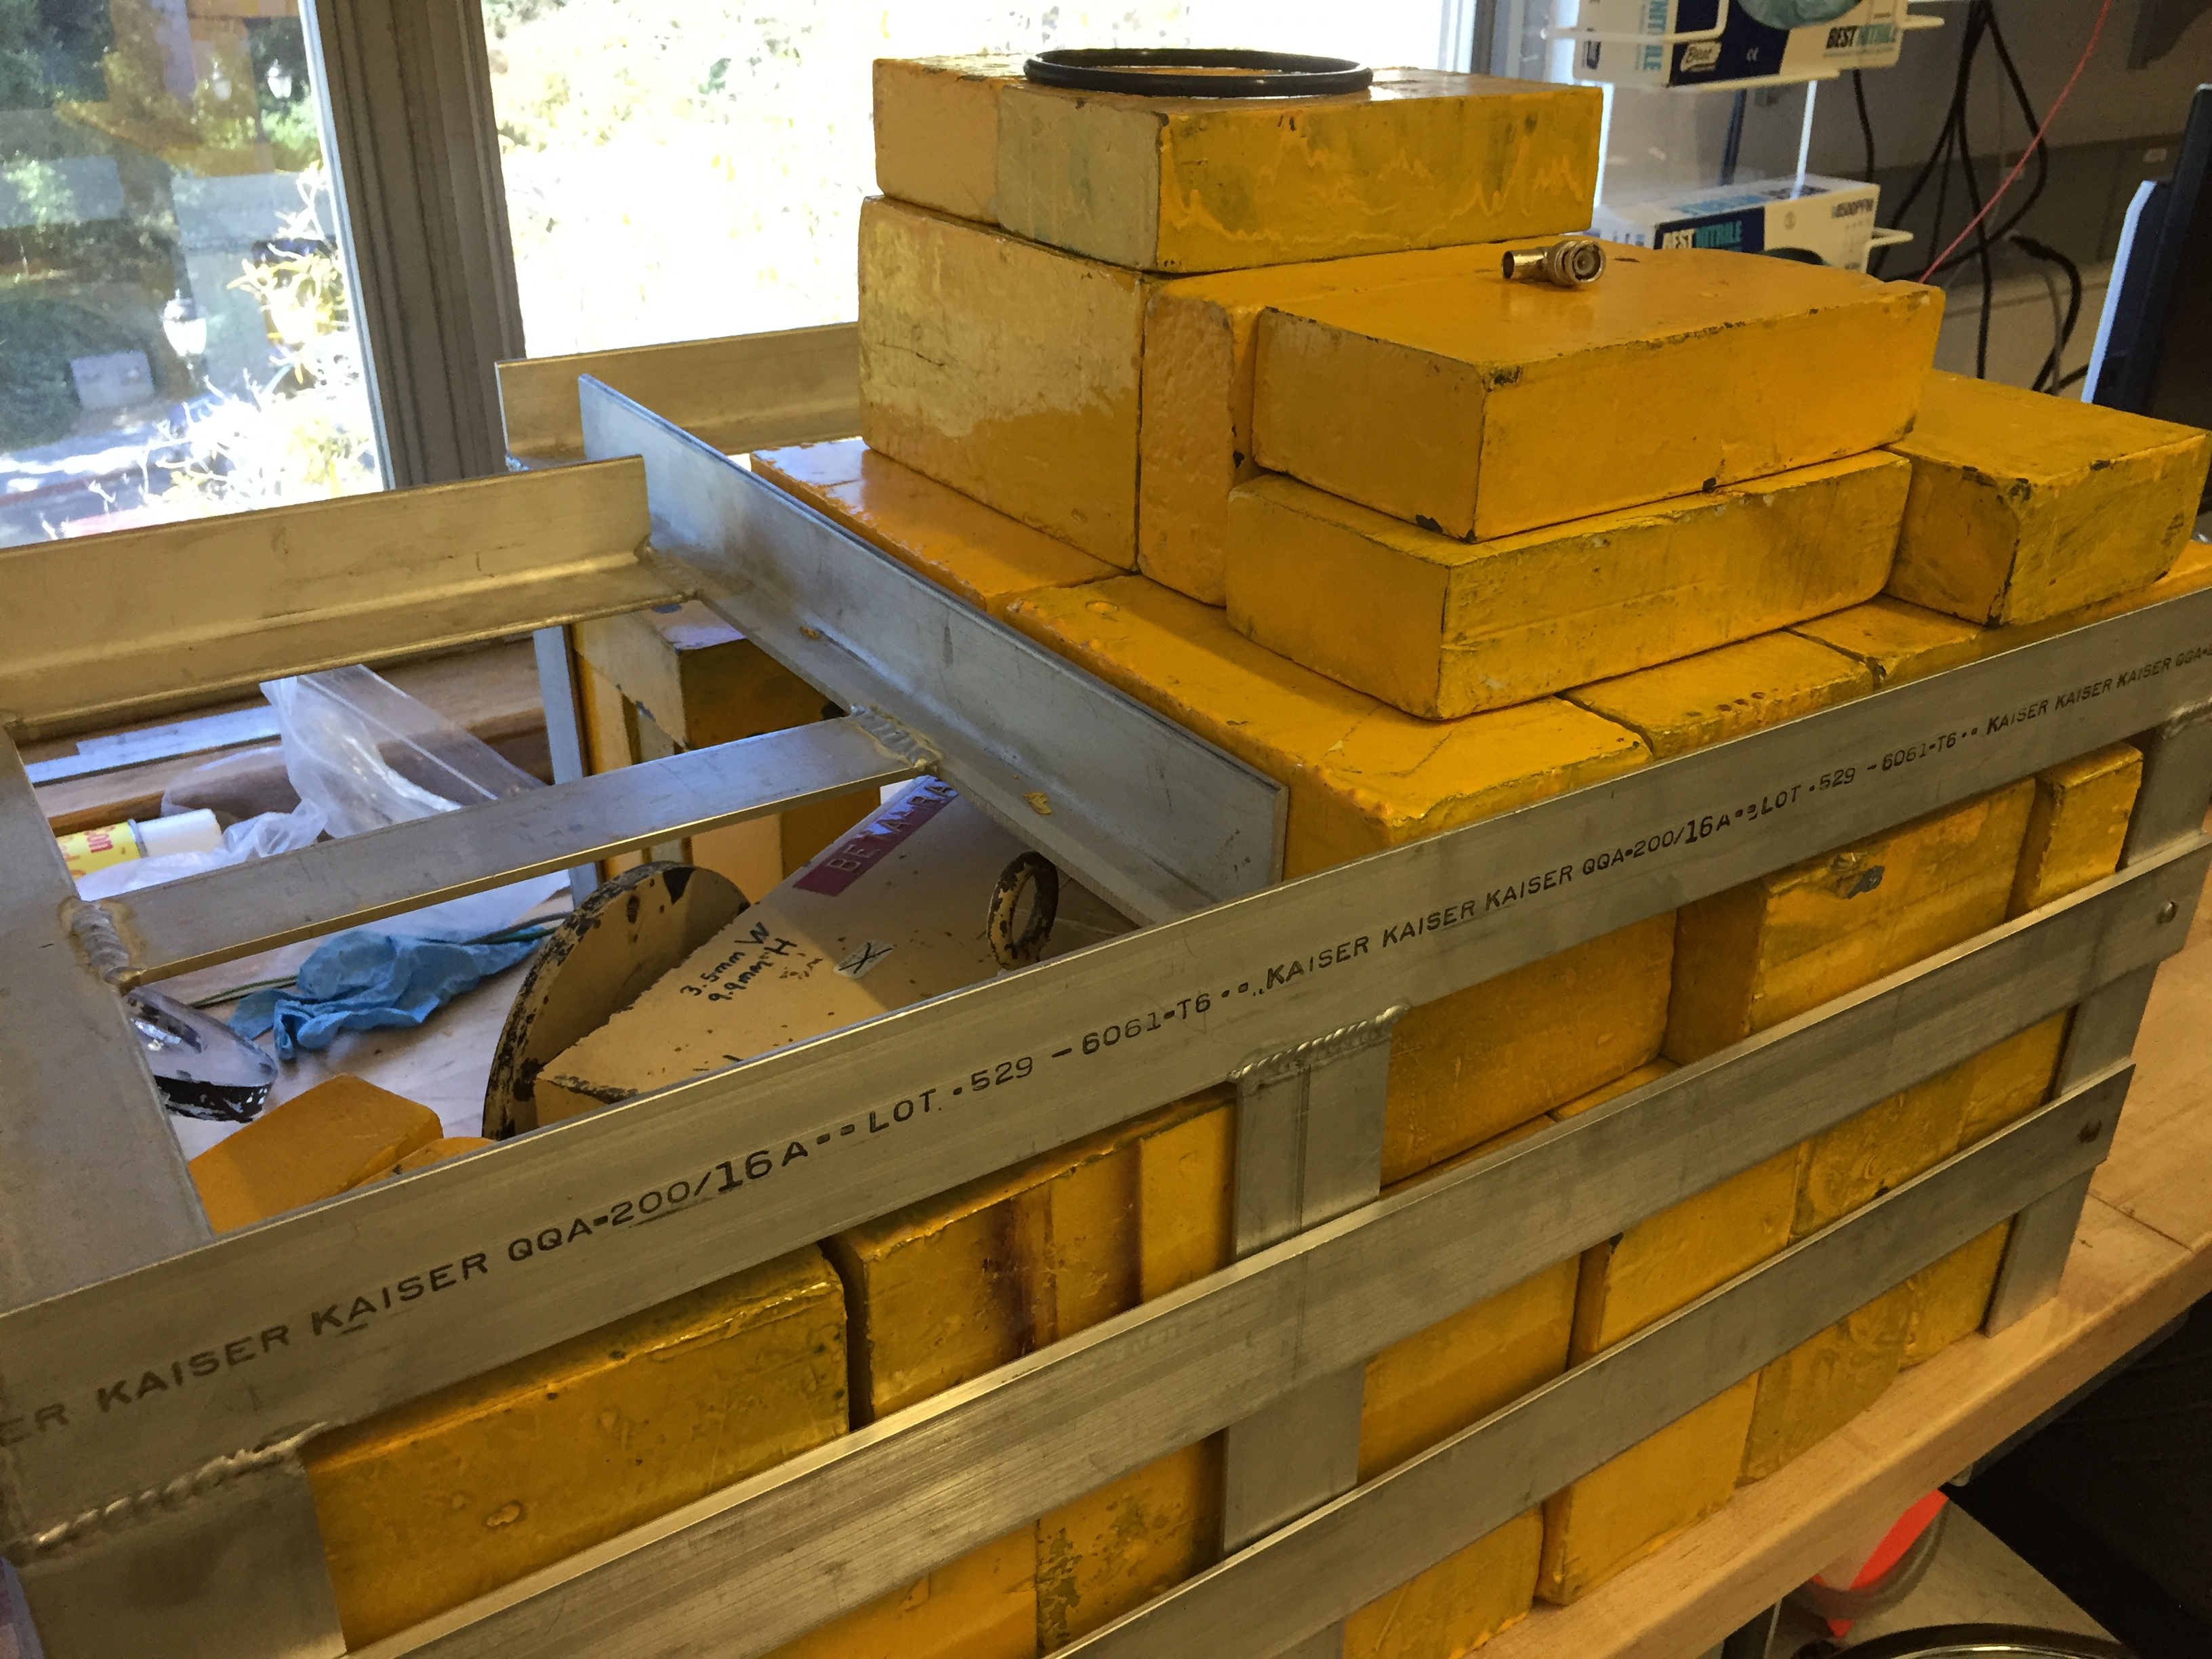
\includegraphics[height=140pt,keepaspectratio]{images/Lead_Brick_Shield.JPG}}
  \caption{Beta Ray Lead\\ Brick Shielding Apparatus \\ \href{http://experimentationlab.berkeley.edu/sites/default/files/images/Lead_Brick_Shield.JPG}{Click here to see larger picture}}
  \label{fig:BRayBlock}
\endminipage\hfill
\minipage{0.49\textwidth}
\centering
 \href{http://experimentationlab.berkeley.edu/sites/default/files/images/Photomultiplier_Base.JPG}{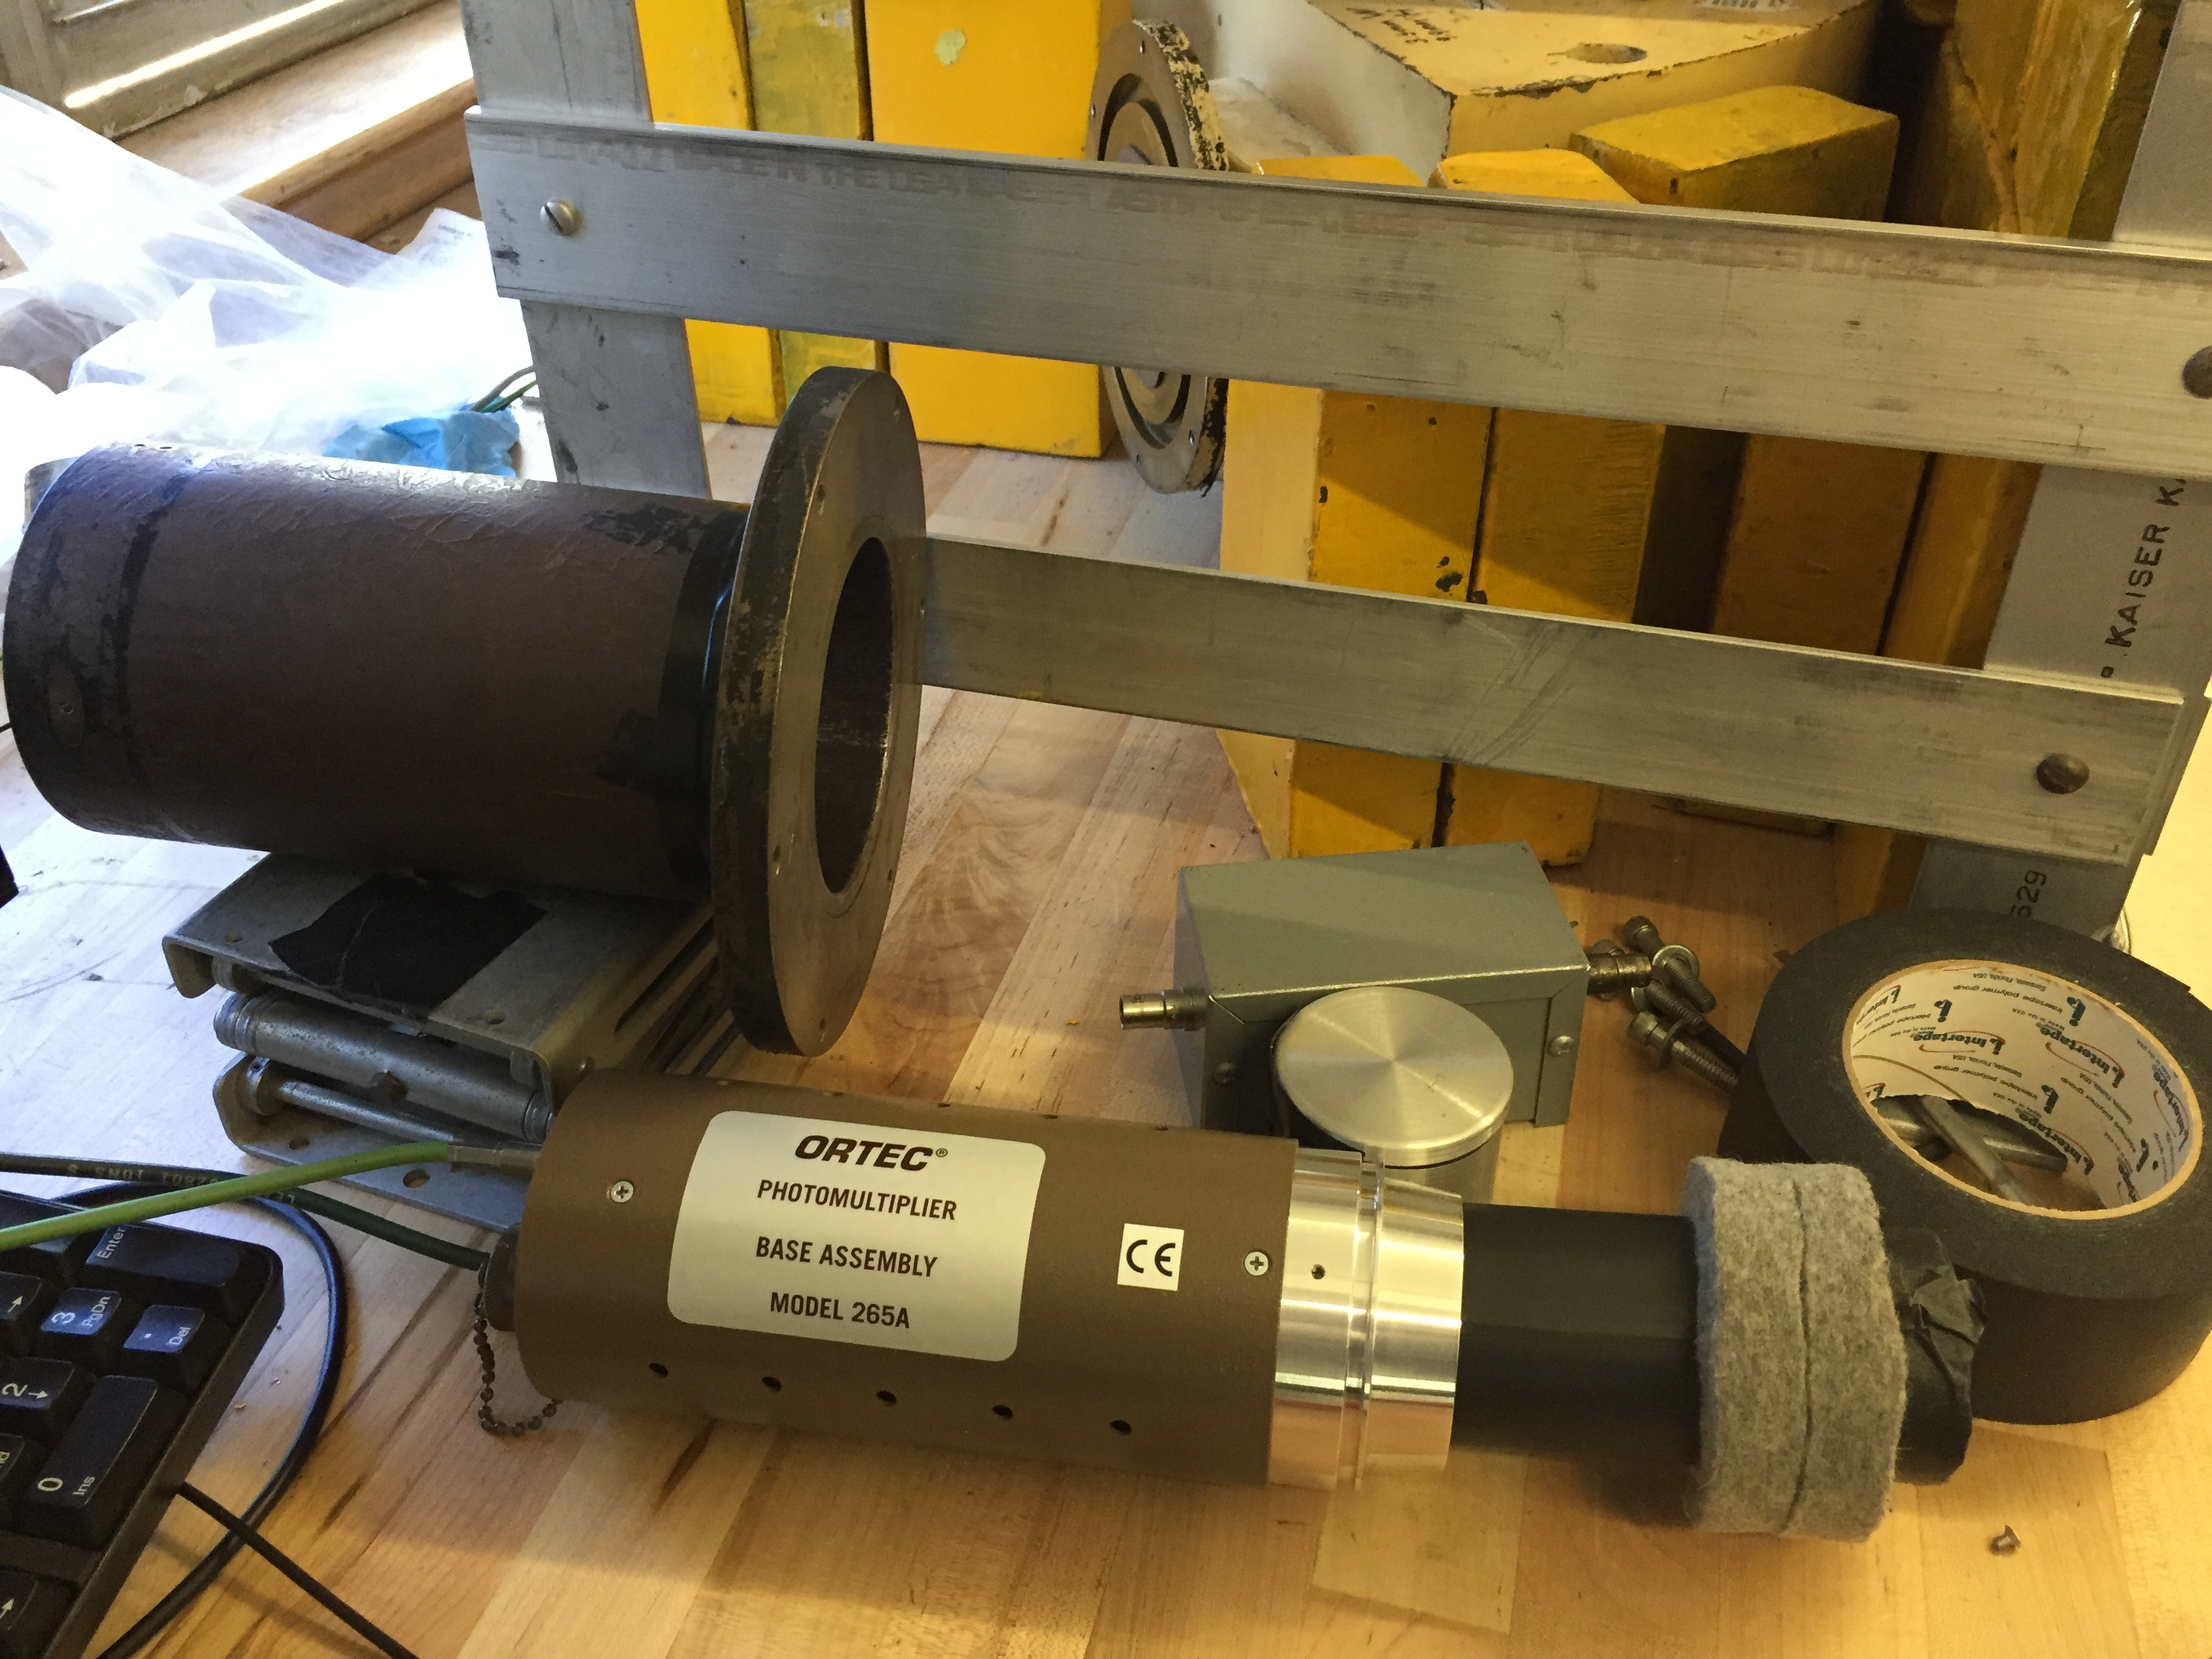
\includegraphics[height=140pt,keepaspectratio]{images/Photomultiplier_Base.JPG}}
  \caption{Photomultiplier \\ Removed from Shielding \\ \href{http://experimentationlab.berkeley.edu/sites/default/files/images/Photomultiplier_Base.JPG}{Click here to see larger picture}}\label{fig:BRayApparatus}
\endminipage
\end{figure}

\section{Before the 1st Day of Lab and SOP for Beta Ray}

\signatures \hyperlink{LabView}{1} \hyperlink{Scope Image}{2} \hyperlink{Statistical Fluctuations}{3} \hyperlink{Hysteresis}{4} \hyperlink{Combined Fermi-Kurie Plot}{5} 

\begin{enumerate}
    \item \emph{\textbf{Note: In order to view the private Youtube videos hosted by the university, you must be signed into your berkeley.edu Google account.}} \\
    View the \href{http://youtu.be/qJ4MPtMmFPw}{\textbf{Beta-Ray Video}}.

    \item \textbf{Radiation Safety SOP} View the \href{http://youtu.be/KHxtzF5pZZM}{\textbf{'Radiation Safety Video'}}. After watching the video in the 111-Lab, get a pink Radiation Safety form from a 111-Lab staff person. Fill it out \& sign the form for getting a \textbf{Radiation Ring}.

    \item Now complete the Radiation Safety Training \href{http://experimentationlab.berkeley.edu/RadiationSafety}{\textbf{Radiation\_Safety}} \textbf{After the training turn in all the forms to Don Orlando or the teaching staff.}

    \item View the \href{\ErrorAnalysisVideo}{\textbf{Introduction to Error Analysis video}} and \href{\ErrorAnalysisNotes}{\textbf{\textbf{Error Analysis Notes}}}.

    \item Read the Standard Operating Procedures (\href{http://experimentationlab.berkeley.edu/sites/default/files/images/SOP\_3271\_Cs-137\_Na-22\_Co-60\_Mn-54\_Am-241\_Fe-55\_2014.pdf}{\textbf{SOP}}) for this lab before starting.

    \item Please fill out the \href{\ExperimentEvaluation}{\textbf{Experiment Evaluation}} and give it to Don Orlando after you finish the lab.

\end{enumerate}

\textbf{Suggested Reading:}

\begin{enumerate}
    \item \href{http://physics111.lib.berkeley.edu/Physics111/Reprints/BRA/04-Table\_for\_Analysis\_of\_Beta\_Spectra.pdf}{\textbf{Tables for the Analysis of Beta Spectra}}; U.S. National Bureau of Standards*

    \item Y. Yoshizawa, ``\href{http://physics111.lib.berkeley.edu/Physics111/Reprints/BRA/Yoshizawa_beta&gammarayspecofCs137.pdf}{\textbf{Beta and Gamma Ray Spectroscopy of Cs137}}'',* Nucl. Phys. \textbf{5}, 122 (1958).

    \item H. A. Bethe, ``\href{http://physics111.lib.berkeley.edu/Physics111/Reprints/BRA/05-Elementary\_Nuclear\_Theory.pdf}{\textbf{Elementary Nuclear Theory}}''.

    \item W. C. Haxton, B. R. Holstein, ``\href{http://physics111.lib.berkeley.edu/Physics111/Reprints/BRA/BRA(state\%20of\%20the\%20science\%20and\%20art\%20of\%20beta\%20decay_OCR\%20.pdf}{\textbf{Neutrino Physics}}'', Am. Jour. Phys. \textbf{68}, 15 (2000).

    \item R. D. Evans, ``\href{http://physics111.lib.berkeley.edu/Physics111/Reprints/R.D.Evans\%20Atomic\%20Nucleus/The\%20Atomic\%20Nucleus\%20Evans\%20full\%20text.pdf}{\textbf{The Atomic Nucleus}}'', McGraw Hill (1972).

\end{enumerate}

* Contained information on the Fermi-Kurie plots and calculations. The reprints are all available on-line from the \href{http://physics111.lib.berkeley.edu/Physics111/Reprints/BRA/BRA\_index.html}{\textbf{Physics 111 Lab Library Site}}.

More \hyperref[sec:References]{References}

You should keep a laboratory notebook. The notebook should contain a detailed record of everything that was done and how/why it was done, as well as all of the data and analysis, also with plenty of how/why entries. This will aid you when you write your report.

\section{Objectives}

\begin{itemize}
    \item Learn what real experimental physics is about.

    \item Learn the synergy between experimental and theoretical work.

    \item Learn to use pieces of equipment that are commonly used in research.

    \item Learn how measurements are performed, analyzed, and interpreted.

    \item Learn how to present your work and results.

    \item Learn problem-solving strategies.

    \item Learn how to manage and organize your time.
\end{itemize}

\section{Introduction}

Some isotopes of a certain element can decay spontaneously and may emit a combination of electrons, positrons, neutrinos, and gamma rays. Nuclei with atomic numbers greater than 80 and a few light isotopes can also emit alpha particles. In this experiment we study the momentum and energy of electrons, called beta particles or beta rays, emitted when radioactive Cesium-137 decays into Barium-137.

\begin{figure}[h]
    \centering
    \href{http://experimentationlab.berkeley.edu/sites/default/files/images/300px-BRAimage003.gif}{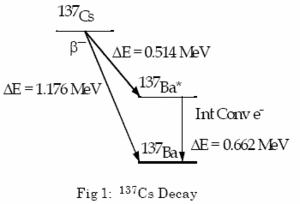
\includegraphics[width=0.5\linewidth]{images/300px-BRAimage003.png}}
    \caption{Cesium decay}
    \label{fig:300px-BRAimage003}
\end{figure}

There are two modes of decay because the barium nucleus has two different energy states to which transitions are allowed. The decay process, kinetic energies released, and the branching ratios (relative frequency of occurrence) of these two beta decays of cesium-137 are shown as follows:
\begin{align}
    \label{eq:Decay1}
    ^{137}\text{Cs} &\rightarrow {}^{137}\text{Ba}^* + \beta^- + \bar{\nu}_e
        & \Delta E &= 0.514 \text{ MeV}
        & \text{BR: } 94.7\% \\
    \label{eq:Decay2}
    ^{137}\text{Cs} &\rightarrow {}^{137}\text{Ba} + \beta^- + \bar{\nu}_e
        & \Delta E &= 1.176 \text{ MeV}
        & \text{BR: } 5.3\%
\end{align}
Additionally, the excited state of Barium $^{137}$Ba$^*$ (daughter product in \eqref{eq:Decay1}), can subsequently decay as follows:
\begin{align}
    \label{eq:Decay3}
    ^{137}\text{Ba}^* &\rightarrow {}^{137}\text{Ba} + \gamma
        & \Delta E &= 0.662 \text{ MeV}
        & \text{BR: } 90\% \\
    \label{eq:Decay4}
    ^{137}\text{Ba}^* + e_\text{bound}^- &\rightarrow {}^{137}\text{Ba} + e_\text{unbound}^- + \text{KE}_\text{electron}
        & \Delta E &= 0.662 \text{ MeV}
        & \text{BR: } 10\%
\end{align}
In \eqref{eq:Decay3}, the $^{137}$Ba$^*$ decays by emitting a 0.662 MeV $\gamma$-ray, In \eqref{eq:Decay4}, the excited barium nucleus decays by interacting with a nearby bound electron in a process called \emph{internal conversion}.

The two beta-decays give a continuous energy spectrum of the emitted electrons, while the internal conversion reaction gives sharp k-, l- and m-peaks in energy (page 125 in the reprints). Figure \ref{fig:CountsVsMomentumUncompensated} is a representative spectrum. It is a plot of the number of electrons N vs. momentum p. The curve is the sum of the three decays described above that emit electrons. The peak on the low energy side of the k-peak is an artifact of the apparatus.

\begin{figure}[h]
\captionsetup{justification=centering}
\begin{minipage}[t]{.5\textwidth}
    \centering
    \href{http://experimentationlab.berkeley.edu/sites/default/files/images/BRAimage008.gif}{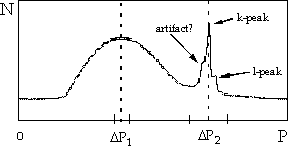
\includegraphics[height=100pt,keepaspectratio]{images/BRAimage008.png}}
    \caption{Counts vs. Momentum, Uncompensated}
    \label{fig:CountsVsMomentumUncompensated}
\end{minipage}
\begin{minipage}[t]{.5\textwidth}
    \centering
    \href{http://experimentationlab.berkeley.edu/sites/default/files/images/BRAimage009.gif}{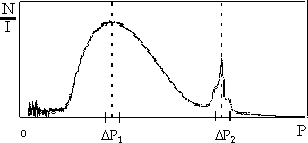
\includegraphics[height=100pt,keepaspectratio]{images/BRAimage009.png}}
    \caption{Counts vs. Momentum, Compensated}
    \label{fig:CountsVsMomentumCompensated}
\end{minipage}
\end{figure}

\section{What is Hysteresis?}

In ferromagnetic materials, microscopic regions are separated into domains. Within each domain, all the atoms have their magnetic moments aligned in one direction. Adjacent domains have their magnetic moments pointing in random directions with respect to their neighboring domains. The sum of the magnetic moments of all the domains is nearly zero (magnetization), and the material produces only a small macroscopic magnetic field.

Domains are separated from each other by ``domain walls'' which are 100 to 1000 atoms wide. Within the boundary of a domain wall, the individual atomic magnetic moments are kind of randomly oriented but sum up to give a net magnetic moment for the domain. When an external magnetic field is applied to the ferromagnetic material, the walls move and the domains with magnetization in the direction of the field increase in size and become macroscopic at the expense of adjacent domains that get smaller and disappear. The combined external field and the field of the ferromagnetic material can be orders of magnitude larger than the external field alone, when all the domains are aligned. This external field is generally supplied by a current-carrying coil wound around the ferromagnetic material.


\begin{figure}[h]
    \centering
    \href{http://experimentationlab.berkeley.edu/sites/default/files/images/BRAimage026.gif}{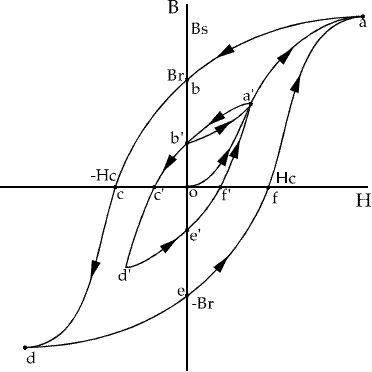
\includegraphics[width=0.5\linewidth]{images/BRAimage026.png}}
    \caption{Hysteresis loop of a ferromagnetic material}
    \label{fig:BRAimage026}
\end{figure}


The degree of magnetization as measured by the size of the domains is non-linearly proportional to the applied external magnetic field. Also, for a given external field, the magnetization of the material depends on its history. For example, start from zero magnetization, and zero external field; increase the external field to any particular value and then reduce it back to zero. The magnetization does NOT return to zero, but remains at some finite value. A reverse external field must be applied to bring the magnetization to zero. The magnetization lags behind the applied field. This effect is known as hysteresis.

A typical but exaggerate hysteresis of a ferromagnetic material is shown in figure \ref{fig:BRAimage026}, where the Magnetic Induction $B$ is plotted versus the Magnetic Field Intensity $H$, which is directly proportional to the applied current in the coil. The horizontal axis could equally well be labeled as ``$I$'' instead of ``$H$''. ``0'' is the non-magnetized or demagnetized state ($B$ = 0, $I$ = 0) which can be reached by applying an alternating current and slowly reducing its amplitude to zero. As the current increases from the demagnetized state, the $B$ value lags behind what one might expect and follows the curve to (a') and toward saturation at (a). With large variations in $I$, the behavior follows a major loop (abcdefa...); while for small variations in $I$, the behavior follows a minor loop (a'b'c'd'e'f'a'...) or (a'b'a'...) if the current $I$ never becomes negative. Certain points of a hysteresis loop have names: Br is the remnant value at $I$ = 0 after the material is saturated at (a.) Hc is the coercive field or the coercivity (i.e. the $H$ or $I$ required to reduce B to zero).

\section{Apparatus}

\begin{figure}[h]
    \centering
    \href{http://experimentationlab.berkeley.edu/sites/default/files/images/600px-BRAimage010.gif}{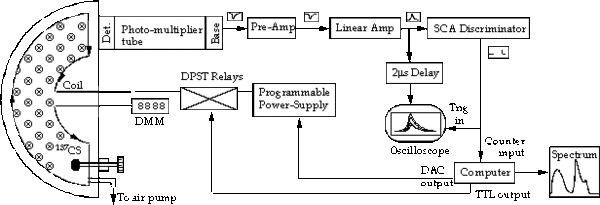
\includegraphics[width=0.5\linewidth]{images/600px-BRAimage010.png}}
    \caption{Diagram of the Beta-Ray apparatus}
    \label{fig:DiagramOfBetaRayApparatus}
\end{figure}

The spectrometer is a `C'-shaped vacuum chamber with conducting coils on top and bottom to produce a uniform magnetic field perpendicular to the horizontal plane of the chamber. The size of the chamber is 0.4375'' x 3.375'' (transverse dimensions). A source of $^{137}$Cs is permanently mounted inside the chamber at one end of a rod (see Figure \ref{fig:DiagramOfBetaRayApparatus} in the `C' diagram). As shown in Figure 3b, the detector is mounted at the other end, behind a slit (0.375'' high x 0.125'' wide). The detector is a piece of 1-inch in diameter plastic scintillator, wrapped with a 2-mil aluminized mylar foil, attached to a 1-1/2 inch diameter light pipe connected to a 6655A photomultiplier tube (PMT).

\begin{figure}[h]
    \centering
    \href{http://experimentationlab.berkeley.edu/sites/default/files/images/BRAimage011.gif}{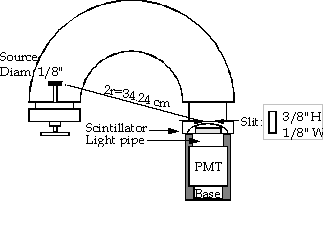
\includegraphics[width=0.5\linewidth]{images/BRAimage011.png}}
    \caption{Diagram showing details of the detector.}
    \label{fig:BRAimage011}
\end{figure}

Electrons emitted by the source are subject to the Lorentz force
\begin{equation}
    q \vec{v} \times \vec {B}
\end{equation}
and travel in a circle to the detector. The relevant equation is:
\begin{equation}
    q_e v B = \frac {m_e v^2}{r}
\end{equation}
The radius r is fixed, and the field $B$ is approximately proportional to the current $I$ in the coils. We can therefore write:
\begin{equation}
    P = m_e v = q_e B r = \text{constant} \times I
\end{equation}
We want to measure the momentum spectrum of the electrons. We can do this by measuring the count $N$ or number of electrons received at the detector in a given time interval, as a function of current $I$.

However, a correction must be applied to N because of the finite size of the slit: The exit aperture is fixed in width and admits a given range of radii, $\Delta r$ = constant. These radii cover a range of momenta $\Delta p$. The magnitude of $\Delta p$ is not constant, but instead increases linearly with $p$, or the current. The plot of $N$ vs. $p$ gives a true representation of the spectrum only if the increasing value of $p$ is compensated or corrected for. Correction is done by dividing each $N$ by the current $I$. An illustration of what happens to the data is shown in Figures \ref{fig:CountsVsMomentumUncompensated} and \ref{fig:CountsVsMomentumCompensated}.

The computer controls the current in the coils, and hence the field. It starts the current from approximately zero and increases it to a maximum in discrete steps called bins or channels. For each bin, the computer counts the number of particles that strike the detector within a period of time and saves these data.

The plastic scintillator produces a light pulse when an energetic electron strikes it. This light is detected by the PMT which produces an electrical pulse with peak-voltage proportional to the energy of the incident beta particle. The pulse is sent through a preamplifier, then a linear amplifier, to a single-channel-analyzer (SCA). The SCA generates a digitized pulse for each detector signal that lies between the adjustable lower and upper thresholds. Because the SCA discriminates against noise pulses, it is also called a discriminator. The digitized pulses are sent to the computer to be recorded in the proper channel of the spectrum. The signal can also be displayed on an oscilloscope.

You should know how the photomultiplier tube works. \href{http://physics111.lib.berkeley.edu/Physics111/Equipment\_Manuals/RCA\_PMT.pdf}{\textbf{Photomultiplier Tube Handbook}}* (Note this is a separate reprint booklet)

Include in your write-up an explanation of the PMT and what the pre-amplifier circuit might look like.

\subsection{Diagram of Photomultiplier Tube}

(See the RCA Photomultiplier Tube Handbook in the Physics Library)\href{http://physics111.lib.berkeley.edu/Physics111/Equipment\_Manuals/RCA\_PMT.pdf}{\textbf{Photo-multiplier tube Handbook}}* (Note: this is a separate reprint booklet.)

We use a 6655A PMT for photon counting.

A Photomultiplier tube is a photon detector that converts single photons into large pulses of electric current by successive multiplying stages.

\begin{figure}[h]
    \centering
    \href{http://experimentationlab.berkeley.edu/sites/default/files/images/BRAimage047.gif}{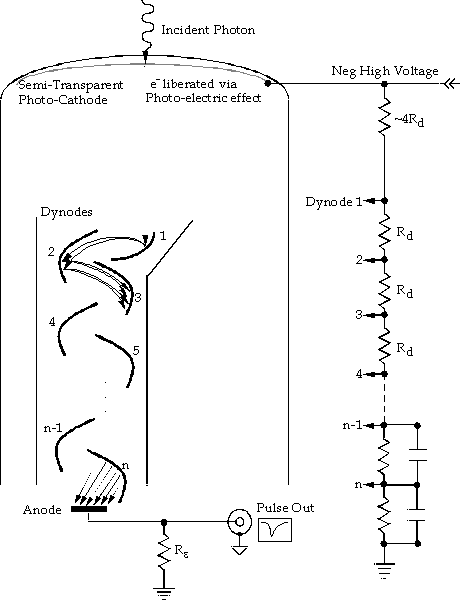
\includegraphics[width=0.5\linewidth]{images/BRAimage047.png}}
    \caption{Diagram of the inside of the Photomuliplier Tubes.}
    \label{fig:BRAimage047}
\end{figure}

\begin{figure}[h]
    \centering
    \href{http://experimentationlab.berkeley.edu/sites/default/files/images/RCA6655A_PMT_3.jpg}{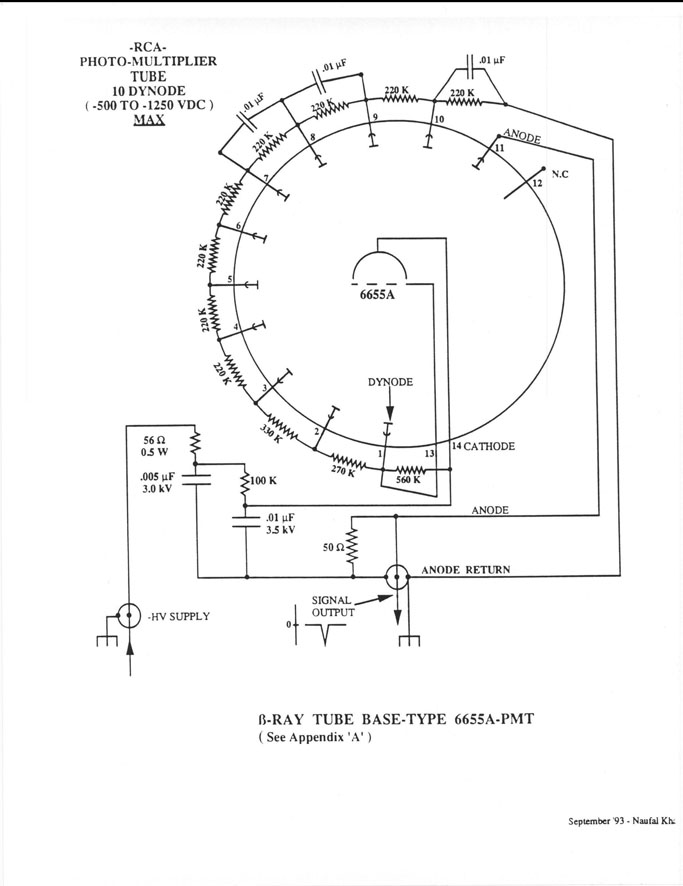
\includegraphics[width=0.5\linewidth]{images/RCA6655A_PMT_3.jpg}}
    \caption{Circuit diagram of the PMT Base.}
    \label{fig:RCA6655A_PMT_3}
\end{figure}

\section{Procedure}

First read and get familiar with the LabView Beta Ray Computer Program  \cite{Siegbahn} which describe the operation of the computerized data-acquisition program that communicates with the DAQ card and controls data taking. The current is supplied to the magnet by a DC power supply in series with a current DVM meter through the relay circuits which can only be set to a particular value with this computer program.

\checkpoint{LabView}{Describe the various components of the LabView program to a GSI and explain how data is collected and what will be measured.}

\subsection{Set the signal and discriminator levels}

\begin{enumerate}
    \item Familiarize yourself with the relationship between the PMT voltage with a maximum of -1100 VDC, amplifier gain, and pulse height. Consult the block diagram of the apparatus (\href{http://experimentationlab.berkeley.edu/sites/default/files/images/BRAimage010.gif}{\textbf{Beta Ray Apparatus}}). The signal path is from the PMT to the current PREAMP (SR570 - Bias Voltage : pos; Filter Type : none; Input Offset : pos, 2 x 100 nA; Filter Freq : not used; Sensitivity : 2 x 1 microA/V) to AMP to a 2 second [DELAY-LINE BOX to SCOPE (when the scope is triggering internally, the delay-line has no effect, but you will need it later to delay the main pulse)], and the Tran-L-Amp Amplifier settings: DIFF DL .8, INT 2, GAIN 16. Referring to a sample spectrum, set the coil current (use the bin setting on the Integrate Single Point Program) to a bin corresponding to a high count rate. Observing the signal on the oscilloscope, gradually turn up the high voltage (negative polarity) on the PMT until an operating voltage of -800 to -1100 V (maximum). You should see many pulses of various heights. Vary the PMT voltage (always between -800 and -1100V max) and the gains of the preamp and the amplifier, and observe the effects on the signal and noise. Change the coil current corresponding to various points on the spectrum and observe how the intensity and height of the pulses change. Note what you see. Remember that you are trying to maximize the signal to noise in the pulses. Set the coil current to approximately 0 amps (bin 0) and observe the signal. Theoretically, there should be no signal at zero field. What do you see, and what can you conclude about the nature of the noise in this experiment? What is the amplitude of the signal at each stage of the processing path?

    You will need to use the ``Signal Point Scan'' for this part before seeing any signals from the apparatus. Refer to section setup of the \hyperref[subsec:IntegrateSinglePointProgram]{Signal Point Scan}

    \item Familiarize yourself with the operation of the SCA: The normal operation of a PMT will result in small-amplitude noise pulses. We want to use the discriminator on the SCA to reduce or eliminate the noise, permitting the signal pulses which are larger in amplitude to be passed and recorded. You can adjust the LLD Lower Level Discriminator or Baseline control to remove the noise line below the pulses. Connect the Tran-L-Amp linear amplifier to the SCA and the rest of the circuit elements as shown in Figure \ref{fig:DiagramOfBetaRayApparatus}, apparatus \href{http://experimentationlab.berkeley.edu/sites/default/files/images/BRAimage010.gif}{\textbf{Beta Ray Apparatus}}. Switch the SCOPE to EXT trigger. Now the scope is only displaying pulses that pass the SCA, and the 2 microsecond (-DELAY-LINE compensates for the SCA's signal transit time.

    \item With the Single Point Program, find a bin that corresponds to a high count on the sample spectrum. This program is a one part of two of the Beta Ray Scan Program Utilities, Beta Ray Computer Program \cite{Krane}. Refer to that section now. Start with the SCA upper-level threshold (UL) set to 10 and the lower-level (LL) set to 0. There should be little or no signal displayed on the SCOPE. Increase the LL until a signal appears on the scope, this is the minimum LL setting you may use (approx. 0.36), the SCA will not operate properly at a lower setting. Now increase LL well past this setting and observe the output on the scope

    \item You should see something similar to Figure \ref{fig:Signal1}. In this case, most of the low voltage noise signals are passing through the discriminator and registering as counts on the computer. Now, by slowly increasing the LL (Lower Level) setting, you should be able to obtain an output similar to Figure \ref{fig:Signal2}. In this picture the lower line and a few of the lower voltage pulses beneath the brightest pulse have been eliminated. This effectively eliminates most of the PMT noise as well as some of the lower momentum pulses.
    
    \checkpoint{Scope Image}{Call a GSI over and show them the image on the scope. Explain what it is that you're seeing.}

    \item The object is to set the LL high enough to eliminate small-amplitude PMT noise while preserving as much of the low-momentum data as you can.

    \begin{figure}[H]
    \captionsetup{justification=centering}
    \minipage{0.32\textwidth}
      \href{http://experimentationlab.berkeley.edu/sites/default/files/images/BRAimage015.jpg}{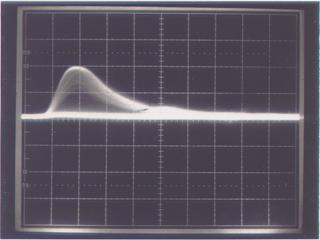
\includegraphics[height=115pt,keepaspectratio]{images/BRAimage015.jpg}}
      \caption{Noisy Signal}
      \label{fig:Signal1}
    \endminipage\hfill
    \minipage{0.30\textwidth}
     \href{http://experimentationlab.berkeley.edu/sites/default/files/images/320px-BRAimage016.jpg}{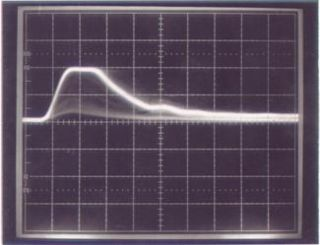
\includegraphics[height=115pt,keepaspectratio]{images/320px-BRAimage016.jpg}}
      \caption{Saturated Signal}
      \label{fig:Signal2}
    \endminipage\hfill
    \minipage{0.32\textwidth}
     \href{http://experimentationlab.berkeley.edu/sites/default/files/images/BRAimage017.jpg}{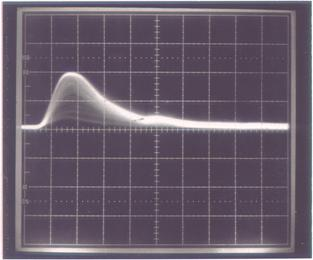
\includegraphics[height=115pt,keepaspectratio]{images/BRAimage017.jpg}}
      \caption{PMT Noise Eliminated}
      \label{fig:Signal3}
      \endminipage
    \end{figure}

    \item The AMP gain should be set around 16, but be careful not to clip the top off your signal. If you set the gain too high on the amplifier it will chip or saturate and look like Figure \ref{fig:Signal2}. Now using the Beta Ray Scan program, take a series of quick spectra (Bins 0-2500 by 10; 3 sec/bin; save time by clicking on the Stop Early Button, click only once, after it has completed taking data in the 'up' direction at about channel \# 2450 (note that the Stop Button takes about 40 second to really stop the program). This should verify your SCA and amplifier settings. With higher LL settings, you should see the lower momentum portion of the spectrum erode. Compare your spectrum to the sample spectrum. If your spectra look too distorted, you may have to repeat step three. Why don't the near-zero-field data disappear with higher discriminator settings?
\end{enumerate}

\subsection{Observe the effects of statistical fluctuations.}

\begin{enumerate}
    \item Using the Integrate Single Bin program acquire 50 or 60 observations each, at one second per integration, for two bins with greatly different count-rates. Save the observations in a file, and use them to calculate the means and standard deviations for the two channels. How do they compare to counting statistics?

    \item For one bin (one single setting of coil-current), observe the change in fluctuation as you change integration times in a range from 1 to 30 seconds.
    
    \checkpoint{Statistical Fluctuations}{Based on the lowest count-rate of all channels, for how long should you integrate each channel of your spectrum to achieve a better than 1\% error due to statistical factors?}

\end{enumerate}

\subsection{Observe the effect of hysteresis}

\begin{enumerate}
    \item Re-read the [\href{http://experimentationlab.berkeley.edu/Hysteresis}{\textbf{hysteresis section}}] and the Analysis section of VI. \textbf{Beta Ray Computer Programs} to be sure that you understand how the scan program establishes a hysteresis loop before it begins taking data.

    \item Take a quick complete spectrum (Bins 0-2000 by 100; 2000-2500 by 5; 2500-4000 by 100; 2 seconds/bin). Observe the shift in the k-peak between the two directions of current. Using the knowledge that the k-peak always occurs at a given magnetic induction (not at a given current), convince yourself that the observed shift in the spectrum between current up and current down is in the correct direction.
    
    \checkpoint{Hysteresis}{Show a GSI this shifting and explain why it demonstrates hysteresis and why it shifts in the direction it does.}

\end{enumerate}

\subsection{Take data using the Beta Ray Scan Program to scan the entire beta ray spectrum}

The current in the magnet is scanned up and down which equals one complete scan. The computer controls the past history of the scans so as to follow the same hysteresis curve every time every time. In adjusting scan parameters, it is more important to integrate for longer times, 60 seconds maximum, than it is to include every point in the spectrum. Print out copies of the scans. We are networked in the 111-LAB so you can choose where to print and what printer to use.

\section{Beta Ray Computer Program}

With the aid of the computer and a LabView program, you can get a rough spectrum in 44 minutes and a full spectrum overnight.

The computer is equipped with an interface DAQ card, PCI-MIO-16E-4, that enables the PC to vary the coil current in either direction from zero to a maximum of approximately 650 mA in 4096 steps. The computer controls the coil current by setting a DAC (digital-to-analog converter) in prescribed steps from 0 to 4095. The DAC outputs its voltage to the power supply that is operating in remote-voltage-controlled \textbf{current} mode. The interface DAQ card also has a edge counter, for counting the beta-particles and background events that strike the detector, and digital TTL-output lines, that permit the PC to switch the current direction. Taken together, these pieces form a 4096-channel particle-momentum spectrum analyzer. The program that operates it is a Labview program entitled \emph{BetaRay Utils.exe``. It will open the two main programs ''BetaRay Scan V2.2`` and ''Single Point Scan V2`` but it will NOT start them. Each of them should be run alone. Wait till one stops before running the other one. If you run both together the LabView will crash. On the Beta Ray computer, this program is accessed by the shortcut on the desktop. If it is not there, look for it under Programs before contacting the 111-Staff.} Data will be saved in your My Documents folder with a pre-name of ''BRA Data`` and ''Single Point" you should add your run \# after this Pre-Name. (ie; BRA Data-1 or Single Point-1)

\subsection{Background Information}

First, it's helpful to define some terms and outline how the system operates. The program can only set the coil-current to fixed values that are determined by the DAC and the power-supply. Each value of current is called a bin or channel. The computer degausses the magnet, sets the current to a bin and then starts counting the number of pulses coming from the detector. This is called integrating a bin. After a period of time, the program stops integrating, takes the number of particles it counted, and moves on to the next bin. After determining the counts for every bin, the program produces a file with entries of Channel Number and counts which constitute a raw spectrum (raw since it is uncompensated for hysteresis effects). The Single Point Program output is Time and Counts. The full Beta Ray Scan program data output file contains Raw Data or Summed Data with the run number and counts. Single Point Scan Program: when you start the program you need to input the channel number first before clicking the start button in the program. The program will then ask you if you are saving the data and for a file name, ie; Single PointXX (you input the XX variable as a run number). Then input the other parameters needed to run the program:

\begin{enumerate}
    \item Base File Path: where your file is being saved and what name the computer gave it.

    \item Status Ring: information on what the program is doing at the time.

    \item Integration Time per Bin: 60 is the maximum number.

    \item Time/Scan Direction: is the time will take to complete the requested up \& down scan.

    \item Estimated Time Remaining: it is updated at the end of each up/down scan with the remaining time.

\end{enumerate}

Note that \textbf{data} is only saved at the completion of each up and down scan. You will see the summed data plot after this time.

This is a good time to point out how your spectra will differ depending on the direction of the changing current. Look at the Figure \ref{fig:Spectrum1} below.

\begin{figure}[h]
\begin{minipage}[t]{.5\textwidth}
    \centering
    \href{http://experimentationlab.berkeley.edu/sites/default/files/images/280px-BRAimage028.gif}{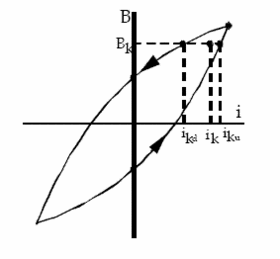
\includegraphics[width=0.9\linewidth,keepaspectratio]{images/280px-BRAimage028.png}}
    \caption{Exaggerated Hysteresis Loop}
    \label{fig:Spectrum1}
\end{minipage}%
\begin{minipage}[t]{.5\textwidth}
    \centering
    \href{http://experimentationlab.berkeley.edu/sites/default/files/images/BRAimage029.gif}{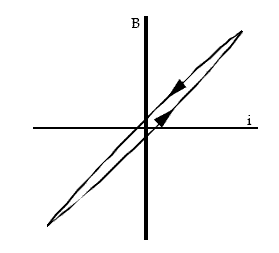
\includegraphics[width=0.9\linewidth,keepaspectratio]{images/BRAimage029.png}}
    \caption{Realistic Hysteresis Loop}
    \label{fig:Spectrum2}
\end{minipage}
\end{figure}

The K-peak of the beta spectrum occurs at a specific field strength, marked $B_k$. If $B$ were directly proportional to the coil-current, the K-peak would always be detected at current $i_k$. Instead, as you take data with the current increasing, the peak occurs at $i_{ku}$, and as the current decreases the peak occurs at $i_{kd}$. This is true for every point of the spectrum, which means that both spectra you take will be shifted away (in opposite directions of $I$) from the spectrum you would get if there were no hysteresis. Figure \ref{fig:Spectrum2} is closer to the real hysteresis curve for the beta spectrometer magnet.

\pagebreak

\subsection{The Beta Ray Scan Program}

\begin{figure}[h]
    \centering
    \href{http://experimentationlab.berkeley.edu/sites/default/files/images/470px-BRAimage030.gif}{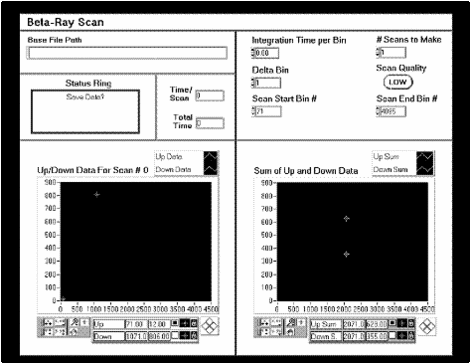
\includegraphics[width=0.5\linewidth]{images/470px-BRAimage030.png}}
    \caption{Scan Program Window}
\end{figure}

Beta Ray Scan is a program that acquires, saves, and plots the number of counts vs. current (bin number), according to the user's input parameters.

Your data will be saved on the 111-Lab server backed up every night by the campus. Data is saved in your own home directory in \textbackslash \textbackslash Atlas2\textbackslash redirect\$\textbackslash your\_Directory\_name\textbackslash My Documents\textbackslash LabVIEW Data\textbackslash then either ``BRA DataXX'' or ``Single PointXX''.

Note you should use Matlab for all your data anlaysis. We have written scripts to help you in you anlaysis. Keep your file names short and desciptive, eg; dataup-1 ending in (.dat), then your data can be read by many other program editors for any changes needed.

The two programs are located on the your desktop. Now at this time please do not run and excute both prgrams at the same time. They will stop working. Do not close them either, just stop them.

After you have started Beta-Ray Scan, you will be asked if you want to save the data that you will be taking. If you choose not to save the data, the data will only be plotted. If you choose to save the data, you will be asked for a file name with the Base File Path as LabVIEW Data\textbackslash BRA Data or Single Point. The program will save raw data points as they are gathered with the file paths:

\textbf{[Base File Path] DOWN data (Raw Data Run \# [Run \#]).xls}

\textbf{[Base File Path] UP data (Raw Data Run \# [Run \#]).xls}

For the Up and Down scan data. The Summed Data will be saved intermittently to the same file with the paths:

\textbf{[Base File Path] DOWN data (Summed Data).xls}

\textbf{[Base File Path] UP data (Summed Data).xls}

For the SUM UP and SUM DOWN data. (Summed data are just that-they are the direct sum of all the previous runs. Think of adding vectors where each component represents a bin number, and the magnitude of that component represents the total number of counts for that bin number).

If you forget where you chose to save the data, don't worry. The Base File Path indicator displays the Base File Path.

Once you have decided whether or not to save the data, you will then have to input the relevant parameters. Here's a list of them and what they do:
\begin{itemize}
    \item Integration Time per Bin(60s Max): Controls the amount of time (in seconds) the computer will sit on each bin tallying the number of counts; e.g., if you choose 5 seconds, the computer will count at each bin for five seconds. Maximum of 60 second for this variable.

    \item Delta Bin: The number of bins the computer will skip (won't integrate) between bins that it integrates.

    \item Number of Up/Down Scans to Make: Each scan consists of data taken as the current increases (UP data) and data taken as the current decreases (DOWN data). And one SUM Total Data file. You should make as many Scans as possible for good data statistics within your time constraints.

    \item Scan Quality: Determines whether or not the computer will wait for the current to settle as it changes bins (while it's taking data). If you select Scan Quality to be HIGH, the computer will wait 4 seconds for the current to settle before it starts integrating the new bin. If you select Scan Quality to be LOW, it won't wait at all. If you want good data, choose a HIGH scan quality.

    \item Scan Start Bin \#: Controls the bin number which the scan will begin taking data at. (The same hysteresis curve will be swept out regardless of the Scan Start Bin.)

    \item Scan End Bin \#: Controls the bin number which the scan will stop taking data at. The actual end bin number is the closest one to the chosen Scan End Bin \# (rounding down) so that the quantity
    \[
    \frac{\text{Scan End Bin} \# - \text{Scan End Bin} \#}{\text{Delta Bin}}
    \]
    is an integer. (The same hysteresis curve will be swept out regardless of the Scan End bin \#.)

    \item Time/Scan Direction: Displays the projected time required for each scan (up and down) to be completed (based on the user inputs) in the format hh:mm:ss. \emph{For example: 1:23:36 requires one hour, twenty-three minutes, thirty-six seconds to complete a scan.}

    \item Estimated Time Remaining: Displays the projected time required to complete the entire scan sequence (i.e. Time/Scan x \# Scans to Make). This indicator updates itself at the end of each scan completed, so it will display the projected time required to finish the total scan sequence (not counting the time required to complete the current scan).

\end{itemize}

\textbf{NOTE}: Ten scans at 5 sec/bin is better than one scan at 50 sec/bin. (Sample values would are below:

Integration Time per Bin (Max of 60 seconds) = 5

Delta Bin = 5

Scans to Make = 7 (could be 6)

Scan Quality = LOW or HIGH add (1/2 second per bin integrated)

Scan Start Bin = 100

Scan End Bin = 4095

Time/Scan = 01:07:01

Total Time = 15:38:14 this gives you an overnight run.

Once all the desired parameters have been entered, click on the flashing [START TAKING DATA] button. Now everything should go as planned. To know what the computer is doing at any given moment, keep an eye on the \emph{Status Ring.}


\begin{figure}[h]
    \centering
    \href{http://experimentationlab.berkeley.edu/sites/default/files/images/BRAimage032.gif}{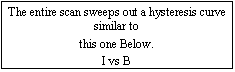
\includegraphics[width=0.5\linewidth]{images/BRAimage032.png}}
    \href{http://experimentationlab.berkeley.edu/sites/default/files/images/BRAimage034.gif}{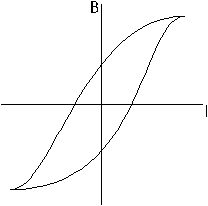
\includegraphics[width=0.5\linewidth]{images/BRAimage034.png}}
    \caption{Depiction of the hysteresis loop you will observe.}
\end{figure}

\begin{enumerate}
    \item The current is set to 0

    \item The current is set to its negative maximum.

    \item The current is returned to 0.

    \item The current is ramped up to that corresponding to the Scan Start Bin \#.

    \item The UP data are taken, stopping at the Scan End Bin \# or thereabouts.

    \item The current is increased to its maximum value.

    \item The current is decreased to that corresponding to the Scan End Bin \# or thereabouts whatever the last integrated bin was in the UP scan.

    \item The DOWN data are taken, stopping at the Scan Start Bin \#.

    \item The current is returned to zero.

    \item The raw UP, DOWN, SUM UP and SUM DOWN data are saved/updated and plotted.

    \item The entire procedure is repeated until all the scans have been made.

\end{enumerate}

During the scan process, you may stop the program pre-maturely by clicking on the [STOP EARLY] button (it will appear after the data run(s) begin). Just click it once. If it seems like it's stuck and won't click, that's probably because the computer is busy integrating a bin and hasn't had time to click it. When it's done integrating that bin, the [STOP EARLY] button will latch. The program may integrate one more bin, then it will stop and bring the magnet through the end of the hysteresis loop once or twice (depending on how many runs were left to complete it takes about 78 seconds to stop). \textbf{You must let it stop normally or the equipment will be left in an unstable condition.} Data taken during the interrupted run will be graphed but not be saved or added to the sum data. (the graph of interrupted down data isn't to be trusted, as the bin numbers won't actually correspond to the points integrated).

\textbf{Note}: Since statistical error decreases with larger samples, longer integration times will give you smoother graphs. Below are two examples of the effect of integration-time on the measured spectrum:

\begin{figure}[h]
    \centering
    \href{http://experimentationlab.berkeley.edu/sites/default/files/images/BRAimage035.gif}{
\includegraphics[width=0.7\linewidth]{images/BRAimage035.png}} \\
    \href{http://experimentationlab.berkeley.edu/sites/default/files/images/BRAimage036.gif}{
\includegraphics[width=0.7\linewidth]{images/BRAimage036.png}}
    \caption{Comparison of Integration-Time on the Spectrum}
\end{figure}

You can see from these graphs (even though their small vertical size slightly obscures their resolution) that the longer the integration time, the smoother the graph. On the other hand, it is not always desirable to take too long an integration time. Sometimes instrumental conditions change over time, and if the last point taken is too far in time from the first point, then the curve does not truly represent the experiment. Ten scans at 5 sec/bin is better than one scan at 50 sec/bin. Take many scans at a lower integration time.

\subsection{The integrate single point program}
\label{subsec:IntegrateSinglePointProgram}

\begin{figure}
\centering
    \href{http://experimentationlab.berkeley.edu/sites/default/files/images/BRAimage037.gif}{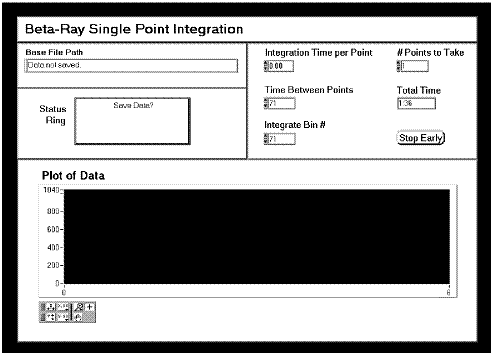
\includegraphics[width=0.7\linewidth]{images/BRAimage037.png}}
    \caption{Integration Program Sample Parameters}
\end{figure}

\textbf{Beta-Ray Single Point Integration} is a program that will sit at a single bin number, magnet current, (determined by the user) and periodically integrate that bin number for a certain amount of time. With this program, one can see how much (if any) instrumental drift there is over long periods of time.

Starting from the computer desktop:

\begin{enumerate}
    \item Double click on the BetaRay Utils (Both VI programs will open, but NOT start running; Single point Integration V2 and Beta Scan V2.2)

    \item Click on the RUN button at the top of the LabView toolbar after you have entered the start bin \#.

\end{enumerate}

\textbf{The following are sample parameters to use:}

\begin{itemize}
    \item Program VI = Beta Ray Single Point Integration

    \item Integration Time per point = 10 (seconds

    \item Time Between Points = 1

    \item Integrate Bin \# = 2200 (the K-peak, enter it before start Run button is clicked)

    \item Number of Points to Take = 60
\end{itemize}

Click on enter (upper left corner) Click on the Run button Question: to SAVE your data or Not to SAVE, your choice.

TOTAL TIME = 00:11:33 (11 minutes and 33 seconds) time enough for you to set the LLD on the discriminator.

To Stop the Program Early, double click on the ``Stop Early'' Button (Note: Button will change to Stopping, wait about 40 seconds for it to stop).

After you have successfully started \emph{Beta-Ray Single Point Integration}, you will be asked if you want to save the data that you will be taking. If you choose not to save the data, the data will only be plotted. If you choose to save the data, you will be asked for a \emph{Base File Path Name}. The program will save the data after the run with the following path:

\textbf{[Base File Path] Single Point-\# Bin Number 2200.xls}

If you forget where you chose to save the data, don't worry. The \emph{Base File Path indicator} displays the \emph{Base File Path}. Once you have decided whether or not to save the data (and where), you will then have to enter the scan parameters. Note that all data saving defaults to the your \textbackslash$\sim$\textbackslash My Documents\textbackslash LabVIEW Data\textbackslash directory.

\begin{itemize}
    \item Integration Time per Point: Sets the amount of time the computer integrates for each data point.

    \item \# Points to Take: Sets the total number of points that will be taken.

    \item Time Between Points: Determines how long the computer will wait after integrating one point before integrating the next point.

    \item Integrate Bin \#: Selects which bin number will be integrated.

    \item Total Time: Displays the total time the procedure will take in the hh:mm:ss format.

\end{itemize}

\emph{For example: Total Time = 11 minutes and 25 seconds (11:25)}

\begin{itemize}
    \item Stop Early: If this button is clicked on, the scan will stop in the middle of the data gathering part (at the end of its integrate/wait sub-cycle), the hysteresis loop will be swept out, and the data will be saved.

\end{itemize}

The \emph{Status Ring} will tell you what the computer is currently doing. The hysteresis cycle that the computer sweeps out is identical to that in the Beta-Ray Scan program. Data will be plotted as they are taken.

\subsection{Analysis}

\subsubsection{Beta-Ray Spectroscopy}

Please see the Matlab program for analysis and the Matlab scripts that have been written for this experiment. The scripts and the executable of Matlab should be in the same working sub-directory so that they can be called inside Matlab; otherwise, you have to use the Matlab command ADDPATH to point to the location of the scripts. Below are descriptions of some calculations.

\begin{itemize}
    \item Please see reference \href{http://physics111.lib.berkeley.edu/Physics111/Reprints/BRA/04-Table\_for\_Analysis\_of\_Beta\_Spectra.pdf}{\textbf{National Bureau of Standards}} about the Fermi-Kurie Transform analysis.

\end{itemize}

You should read and understand about the Fermi-Kurie-Transform analysis. The reprint National Standards will give you all the needed information to understand this operation. See the faculty for more information.

\subsubsection{Shift DataSets}

This command takes two data sets, assumed to be beta spectra, and shifts them toward each other in order to account for hysteresis effects in the 111-Lab beta-spectrometer. You will be prompted for the `UP' and `DOWN' spectrum, at which time you press the alt-key numbers that correspond to the proper data sets. Then you will be asked for the amount to shift. The spectra are then shifted toward each other by means of \emph{x-axis rescaling} (see that section of this manual for more info). That is, the x-axis is rescaled in the same way as the \emph{Calibrate x-axis} low and \emph{Calibrate x-axis} high commands. The shift command is cumulative, if you shift 50 bins and then shift -4 more, you will have a total shift of 46 bins. And the effects of the shift command may be removed with the \emph{Reset x-axis} scaling command applied to each of the two spectra.

\subsubsection{Compensate DataSet}

Compensate DataSet creates a new DataSet from the current one by dividing the y-value of each point by its calibrated (scaled) x-value, i.e.
\[
    \left( x_i, y_i \right) \rightarrow \left( x_i, \frac {y_i}{x_i} \right)
\]
This is useful for processing raw momentum data from the semicircular spectrometer, in which the bin-width is proportional to the bin.

\subsubsection{Fermi-Kurie Transform}

Fermi-Kurie Transform creates a new DataSet that is the Fermi-Kurie plot of the current one [see NBS for complete treatment]. The transform is a theoretical one that changes the DataSet into a straight line. The transformation is:
\[
\left(x_{i},y_{i}\right) \rightarrow \left(\sqrt{x_{i}^{2}+1}-1, \sqrt{\frac{y_{i}}{x_{i}^{2} \cdot F\left(Z,x_{i}\right)}}\right)
\]
where $F(Z, x_{i})$ is the Quantum-mechanical correction for coulomb effects on the beta-particle as it leaves the parent atom. $F(Z, x_{i})$ is calculated using the Bethe-Bacher approximation but the screening effect [ref 3 \S12] is neglected (to see why, you should calculate the size of this effect for $^{137}$Cs). This transformation assumes that the x-axis is momentum and has been calibrated in units of $m_e c$. The resulting x-axis is then kinetic energy in units of $m_e c^{2}$. If the input DataSet begins with negative momenta, \emph{Matlab} will handle this information and begin processing data.

\subsubsection{Inverse Fermi-Kurie Transform}

The inverse Fermi-Kurie feature inverts the previous algorithm producing:
\[
(x_i, y_i) \rightarrow \left(\sqrt{(x_i + 1)^2 - 1}, y_i^2 \left( \left(x_i + 1 \right)^2 - 1 \right) F \left(Z, \sqrt{(x_i + 1)^2 - 1} \right) \right)
\]

\section{Beta Ray Data Analysis}

\subsection{What does artifact mean?}

If you compare the spectrum taken in this lab to ones taken elsewhere, you will find in your spectrum, an extra peak on the lower momentum side of the k-peak (see Figure \ref{fig:RawSpectrum} ``artifact''). Before we automated the scan process with a computer, the current in the magnet was adjusted by hand, and it was impossible to obtain the resolution necessary to see this anomaly. But now, with the advent of the computer, intrinsic errors in the beta ray spectrometer have become apparent.

\begin{figure}[h]
\captionsetup{justification=centering}
    \centering
    \href{http://experimentationlab.berkeley.edu/sites/default/files/images/BRAimage039.jpg}{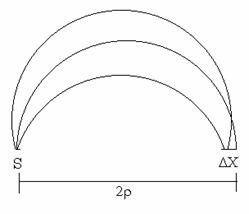
\includegraphics[width=0.5\linewidth]{images/BRAimage039.jpg}}
    \caption{Source of width S emits electrons into a uniform \\magnetic field results in an impact pattern of width $\Delta$X}
    \label{fig:BRAimage039}
\end{figure}

To understand this, consider a source of finite width $s$ emitting a monochromatic beam of $\beta$-rays subject to a uniform transverse magnetic field. Rays (electrons) are emitted in all directions. However, due to the Lorenz force they are confined to travel along arcs of the same radius $r$. Each electron travels along identical arcs, but not the same distance. Thus a detector of width $\Delta x$ ``sees'' an intensity distribution similar to that of Figure \ref{fig:TheoreticalErrorFunction}. This implies that in the experiment, when a polychromatic beam is emitted and one ``sits'' at a bin and counts electrons, the count is smaller than it should be, because some electrons are falling into neighboring bins, due to the width of the intensity distribution. In essence our raw spectrum is the result of what we should see (the true spectrum) with this distribution (the error function) smeared into it. Mathematically this is known as convolution. We would write
\[
G = T \times E
\]

\begin{figure}[h]
    \centering
    \href{http://experimentationlab.berkeley.edu/sites/default/files/images/BRAimage040.gif}{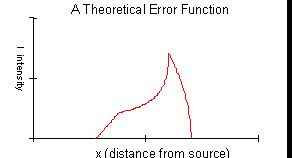
\includegraphics[width=0.5\linewidth]{images/BRAimage040.png}}
    \caption{Theoretical Error Function}
    \label{fig:TheoreticalErrorFunction}
\end{figure}

So can we mathematically deconvolute our data and find the true spectrum? Yes in some special cases, but not here because the error function is not a constant width as we vary B and take our data. Also, the data are not accurate enough to warrant a detailed mathematical treatment. Instead, we smooth the curve by hand and eye in the region where there is an extra bump on the side of the peak, and proceed with the analysis.

\begin{figure}[h]
    \centering
    \href{http://experimentationlab.berkeley.edu/sites/default/files/images/BRAimage041.gif}{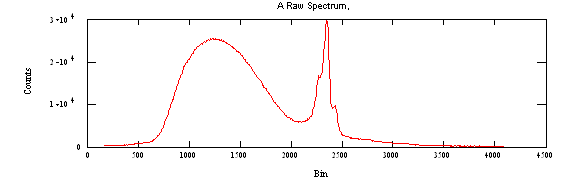
\includegraphics[width=0.5\linewidth]{images/BRAimage041.png}}
    \caption{Note the ``artifact'' peak to the\\ left of the k-peak at Bin \# 2200; see Figure \ref{fig:CountsVsMomentumUncompensated}}
    \label{fig:RawSpectrum}
\end{figure}

So now we can deconvolute our data and find our true Beta spectrum. Figure \ref{fig:DeconvolutedRawSpectrum} is our resultant Beta spectrum, see the K-peak at Bin \# 2200 and L-peak to the right of it.

\begin{figure}[h]
    \centering
    \href{http://experimentationlab.berkeley.edu/sites/default/files/images/BRAimage042.gif}{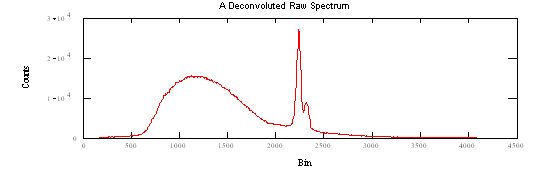
\includegraphics[width=0.5\linewidth]{images/BRAimage042.png}}
    \caption{Resultant Beta Spectrum, see K-peak \\at Bin \#2200 and L-peak to the right of it}
    \label{fig:DeconvolutedRawSpectrum}
\end{figure}

\section{Data Analysis and Fermi-Kurie Plots}

This section use the \href{http://experimentationlab.berkeley.edu/matlabfitting}{\textbf{Matlab scripts}} The Fermi-Kurie plot is simply an algorithm that transforms your spectrum to another view of the energy spectrum. It uses the formula [B10] in the National Bureau of Standards reference. The expectation of this experiment is to experimentally determine $Q_1$ and $Q_2$ , respectively the high and low energy 'X' intercept points. FK (Fermi-Kurie ) transform makes it easier to determine $Q_1$ and $Q_2$ . First you must start with your full data spectrum from channel 0 to 4095 summed up and down data shifted together and then compensated, calibrated, and background-subtracted. Make a Folder in your My Documents folder for your data saving. Save your data ending in \*.DAT. The Excel files need to be opened and re-saved as ``Text delimited with Tab'' files ending in \*.DAT. After you have acquired your data, using the summed up and summed down files save them as the Fileup1.dat and filedn1.dat in excel as ``Text delimited with Tab'' files. Shift them together by the your calculated number, (see \href{http://experimentationlab.berkeley.edu/matlabfitting}{\textbf{Matlab scripts)}} if they look okay then go on with the analysis.

If they are not perfect with respect to the hysteresis effects, then you will have to adjust the data yourself. You will need to shift each Y value by the different between the Y's at each X. In some instances you will have to average the Y's.

Then take your data and subtract background, Watch for negative numbers adjust if needed. Calibrate your X-axis, low and high points for momenta and compensate it ``$Q$'' in Matlab.

Save this dataset file as a new dataset in Matlab. You will want to save the files as you go to each step. Good practice in case of computer crashes, etc. Note that you can save files in ASCII or Binary format.

Now you are ready for generating the Fermi-Kurie plot;

Crop out unwanted bad data points like negative numbers, etc with the use of markers. The Fermi-Kurie plot that you should get is something like the below graph.
\begin{figure}[h]
\centering
    \href{http://experimentationlab.berkeley.edu/sites/default/files/images/BRAimage019.gif}{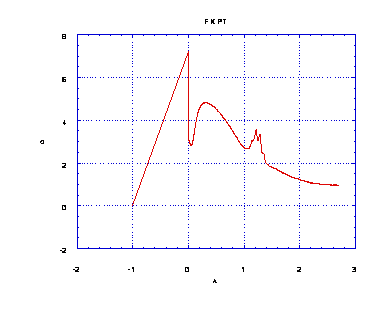
\includegraphics[width=0.5\linewidth]{images/BRAimage019.png}}
    \caption{Sample Fermi-Kurie Plot}
\end{figure}

Fit a line to this curve and get the end-point on the X-axis, $Q_1$. Pick a region above the noise and above the K-peak where it is linear. Now do a inverse Fermi-Kurie plot. You will get something like Figure \ref{fig:021}.

You should repeat the steps above to get the low-energy component and the low-energy end-point $Q_2$. Your result should be the low-energy component as seen in Figure \ref{fig:020}.

\begin{figure}[h]
\captionsetup{justification=centering}
\begin{minipage}{0.32\linewidth}
    \href{http://experimentationlab.berkeley.edu/sites/default/files/images/BRAimage021.gif}{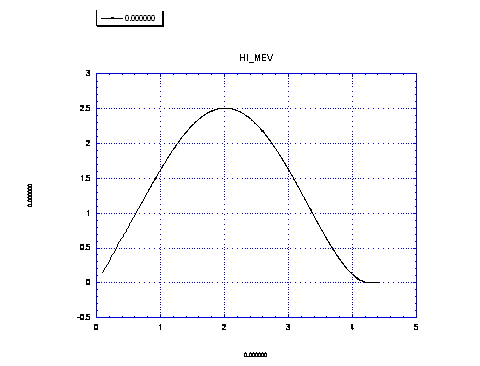
\includegraphics[width=\linewidth]{images/BRAimage021.png}}
    \caption{High Energy}
    \label{fig:021}
    \end{minipage} \hfill
    \begin{minipage}{0.32\linewidth}
    \href{http://experimentationlab.berkeley.edu/sites/default/files/images/480px-BRAimage020.gif}{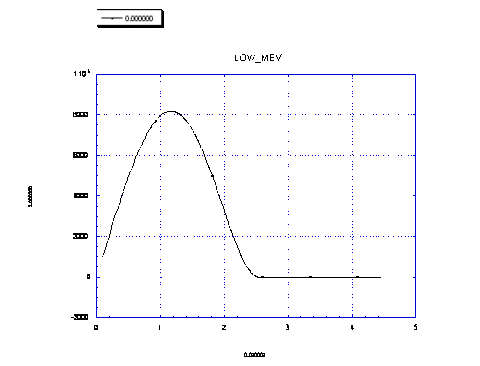
\includegraphics[width=\linewidth]{images/480px-BRAimage020.png}}
    \caption{Low Energy}
    \label{fig:020}
    \end{minipage} \hfill
    \begin{minipage}{0.32\linewidth}
        \href{http://experimentationlab.berkeley.edu/sites/default/files/images/BRAimage022.gif}{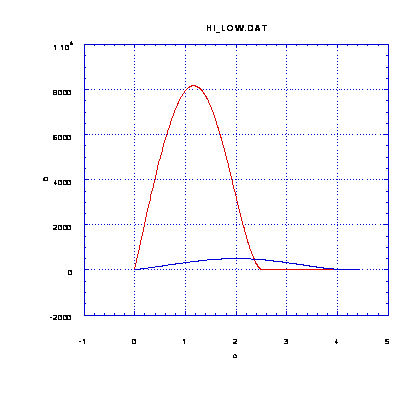
\includegraphics[width=0.8\linewidth]{images/BRAimage022.png}}
    \caption{Combined Graph}
    \label{fig:Combined}
    \end{minipage}
\end{figure}

Your combined graphs should be like Figure \ref{fig:Combined}:

\checkpoint{Combined Fermi-Kurie Plot}{Show your combined graph to a GSI.}

%\textbf{Checkpoint: Show your combined graph to a GSI.}

Reduce your data by following the numbered steps listed below, but first read Ref. 1 for detailed explanations of how beta-ray spectra are analyzed. Also read about data analysis.

In your Fermi-Kurie analysis, use units of $\eta \equiv \frac {p}{m_e c}$ and $\epsilon \equiv \frac{E}{m_e c^2}$ for momentum and energy respectively.

As you work on the data, keep in mind what your ultimate goals are: To observe the beta decay spectrum; to model the phenomenon with a Fermi-Kurie plot that incorporates the theory of beta decay; to determine the maximum energy available in the decay process. Figure \ref{fig:FermiKuriePlot} shows four separate phenomena. Your data is the sum of these. We would like to separate this sum into the individual curves shown above, where they are shown overlapping but not added, as they are in the experimental data. See Appendix D about the Fermi-Kurie plot

\begin{enumerate}
    \item From the masses of $^{137}$Ba and $^{137}$Cs, calculate the total energy available to the electron mass energy + electron kinetic energy + neutrino energy in the beta decay. What is the maximum kinetic energy with which the $^{137}$Ba can recoil? Must this kinetic energy be taken into account in your experiment?

    \item Use Matlab for combining your MYDATUP1.DAT and MYDATDN1.DAT files to reduce the effects of hysteresis and to yield a single data file which you will use in all your analyses. Should you add the two sweeps? Should you displace the two spectra by a constant amount or a variable amount? Should you shift them right or left an amount that depends on channel number? Some thought and justification are needed here. Plot your two raw spectra and your combined spectrum.
          
    \begin{figure}[h]
    \centering
        \href{http://experimentationlab.berkeley.edu/sites/default/files/images/BRAimage025.gif}{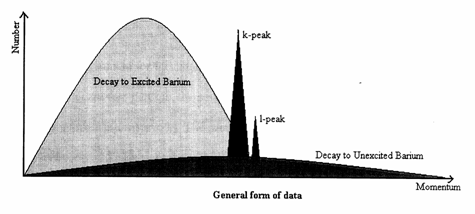
\includegraphics[width=0.5\linewidth]{images/BRAimage025.png}}
        \caption{Fermi-Kurie Plot}
        \label{fig:FermiKuriePlot}
    \end{figure}

    \item The momentum resolution $\Delta p$ is proportional to the momentum p itself (you should derive this), and therefore, $\Delta p$ is proportional to the current, since $I$ is proportional to $p$. Divide the number of counts in each channel of your combined spectrum by $I$ (or a number proportional to $I$). This is your \emph{compensated momentum spectrum} Nc. Plot Nc vs. $\eta$.

    \begin{enumerate}
        \item Calibrate your momentum scale in units of $\eta$ by using the accepted value of the k-peak momentum (KE $\cong$ 624 keV, or $\eta \cong$ 1.98 $m_e c$), the bin in which the k-peak appears, and the bin number that corresponds to zero B-field (and hence zero momentum). Without accounting or correcting for hysteresis effects, how large an error in momentum would you have unwittingly obtained for the k-conversion electron momentum?

        \item Use the region of your spectrum that lies above the highest-momentum beta-particle to estimate the background radiation (you may assume the background is linear) and subtract it from your data. Plot the resultant spectrum.

        \item Make a Fermi-Kurie plot of your compensated spectrum. If the data were perfect, and the theory exact, then the F-K plot would be a straight line. Using a least-squares-fit line, determine the end-point of the high-energy beta component. How would the end-point plot change if the neutrino did not have zero rest mass? This need not be a mathematical explanation and Appendix F, for comments about error analysis.

        \item By taking the inverse-Fermi-Kurie plot of the best-fit line obtained above you will have the contribution of the high-energy beta-component to your compensated spectrum (Nc). Subtract the higher energy component from your compensated spectrum to leave only the lower-energy component.

        \item Make a Fermi-Kurie plot of the subtracted spectrum in the vicinity of the end-point of the lower-energy beta spectrum. Determine the end-point of the low-energy component.

        \item Compare the measured line width and the expected spectrometer resolution for the conversion electron peak.

        \item Check out \href{\ErrorAnalysisNotes}{\textbf{\textbf{Error Analysis Notes}}} and the video on Error Analysis.

        \item Last day of the experiment please fill out the \href{\ExperimentEvaluation}{\textbf{Experiment Evaluation}}

    \end{enumerate}

\end{enumerate}

Copyright 2017 The Regents of the University of California. All rights reserved.

\begin{thebibliography}{}
\label{sec:References}
    \bibitem{Siegbahn} M. Siegbahn, \href{http://physics111.lib.berkeley.edu/Physics111/Reprints/BRA/02-Beta\_Ray\_Spectrometer.pdf}{\textbf{Beta and Gamma Spectroscopy}}, Ch. 3.*

    \bibitem{Krane} K. S. Krane,``\href{http://physics111.lib.berkeley.edu/Physics111/Reprints/BRA/03-Beta\_Decay.pdf}{\textbf{Beta Decay}}.'' Introductory Nuclear Physics, Chapter 9, pp.272-288. John Wiles and Sons., 1987.

    \bibitem{PhotoMultiplierTubeHandbook} \href{http://physics111.lib.berkeley.edu/Physics111/Equipment\_Manuals/RCA\_PMT.pdf}{\textbf{Photo-multiplier tube Handbook}}* (Note this is a separate reprint booklet)

    \bibitem{Feister} I. Feister, ``\href{http://physics111.lib.berkeley.edu/Physics111/Reprints/BRA/Feister_EvaluationoftheFermiBeta-DistributionFunction.pdf}{\textbf{Numerical Evaluation of the Fermi Beta-Distribution Function}}'', Physical Review 78, 4 (1950) *\*.

    \bibitem{Elton} L.R.B. Elton, ``\href{http://physics111.lib.berkeley.edu/Physics111/Reprints/BRA/Elton\_Nuclear\%20Theory\%20Ch.\%209\%20Beta\%20Decay.pdf}{\textbf{Chapter 9: Beta Ray Theory}}'', Introductory Nuclear Theory, 2nd ed.; 1966, W.B. Saunders Company,PA
\end{thebibliography}

Other reprints and reference materials can be found on the \href{http://physics111.lib.berkeley.edu/Physics111/Reprints/BRA/BRA\_index.html}{\textbf{Physics 111 Library Site}}

\end{document}
